\section{Qsim::Params Class Reference}
\label{classQsim_1_1Params}\index{Qsim::Params@{Qsim::Params}}
{\tt \#include $<$qsim.h$>$}

Inheritance diagram for Qsim::Params:\nopagebreak
\begin{figure}[H]
\begin{center}
\leavevmode
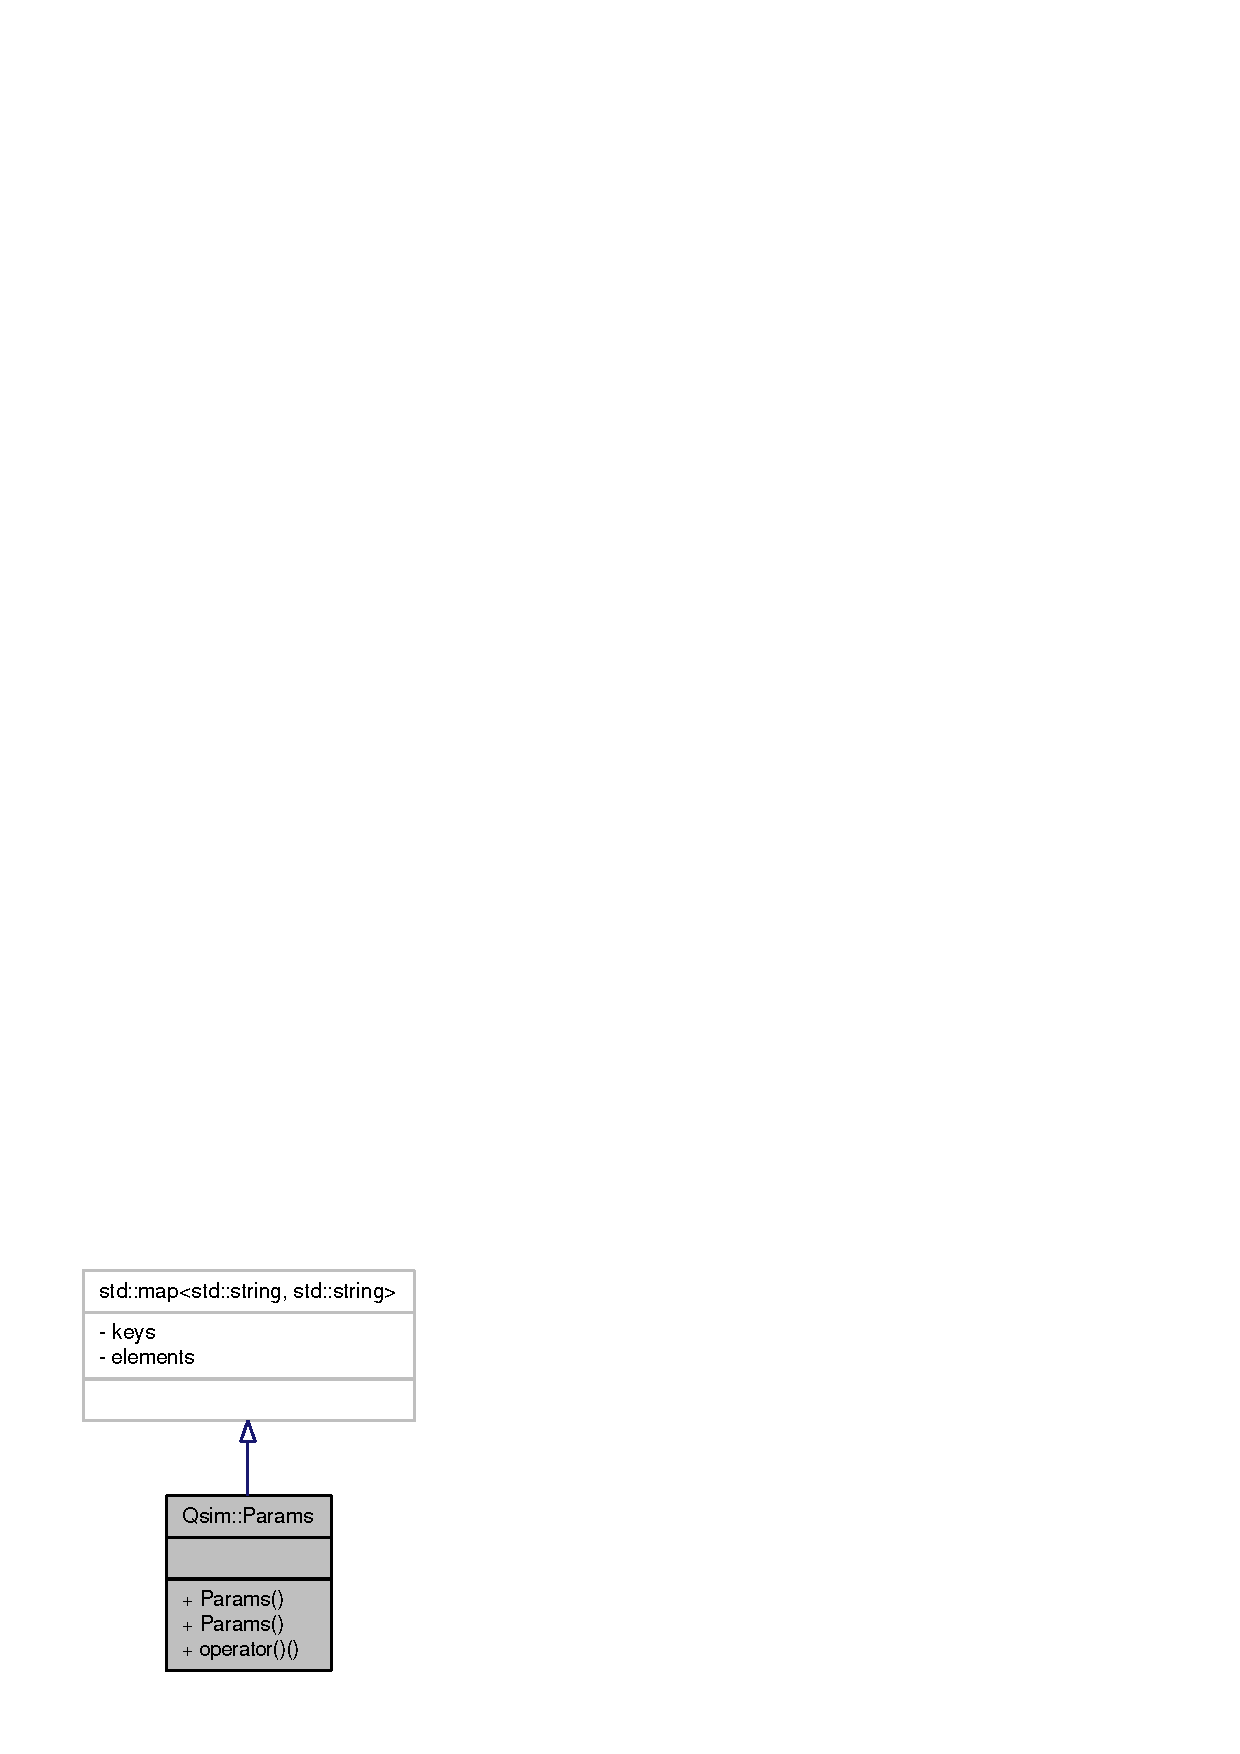
\includegraphics[width=202pt]{classQsim_1_1Params__inherit__graph}
\end{center}
\end{figure}
Collaboration diagram for Qsim::Params:\nopagebreak
\begin{figure}[H]
\begin{center}
\leavevmode
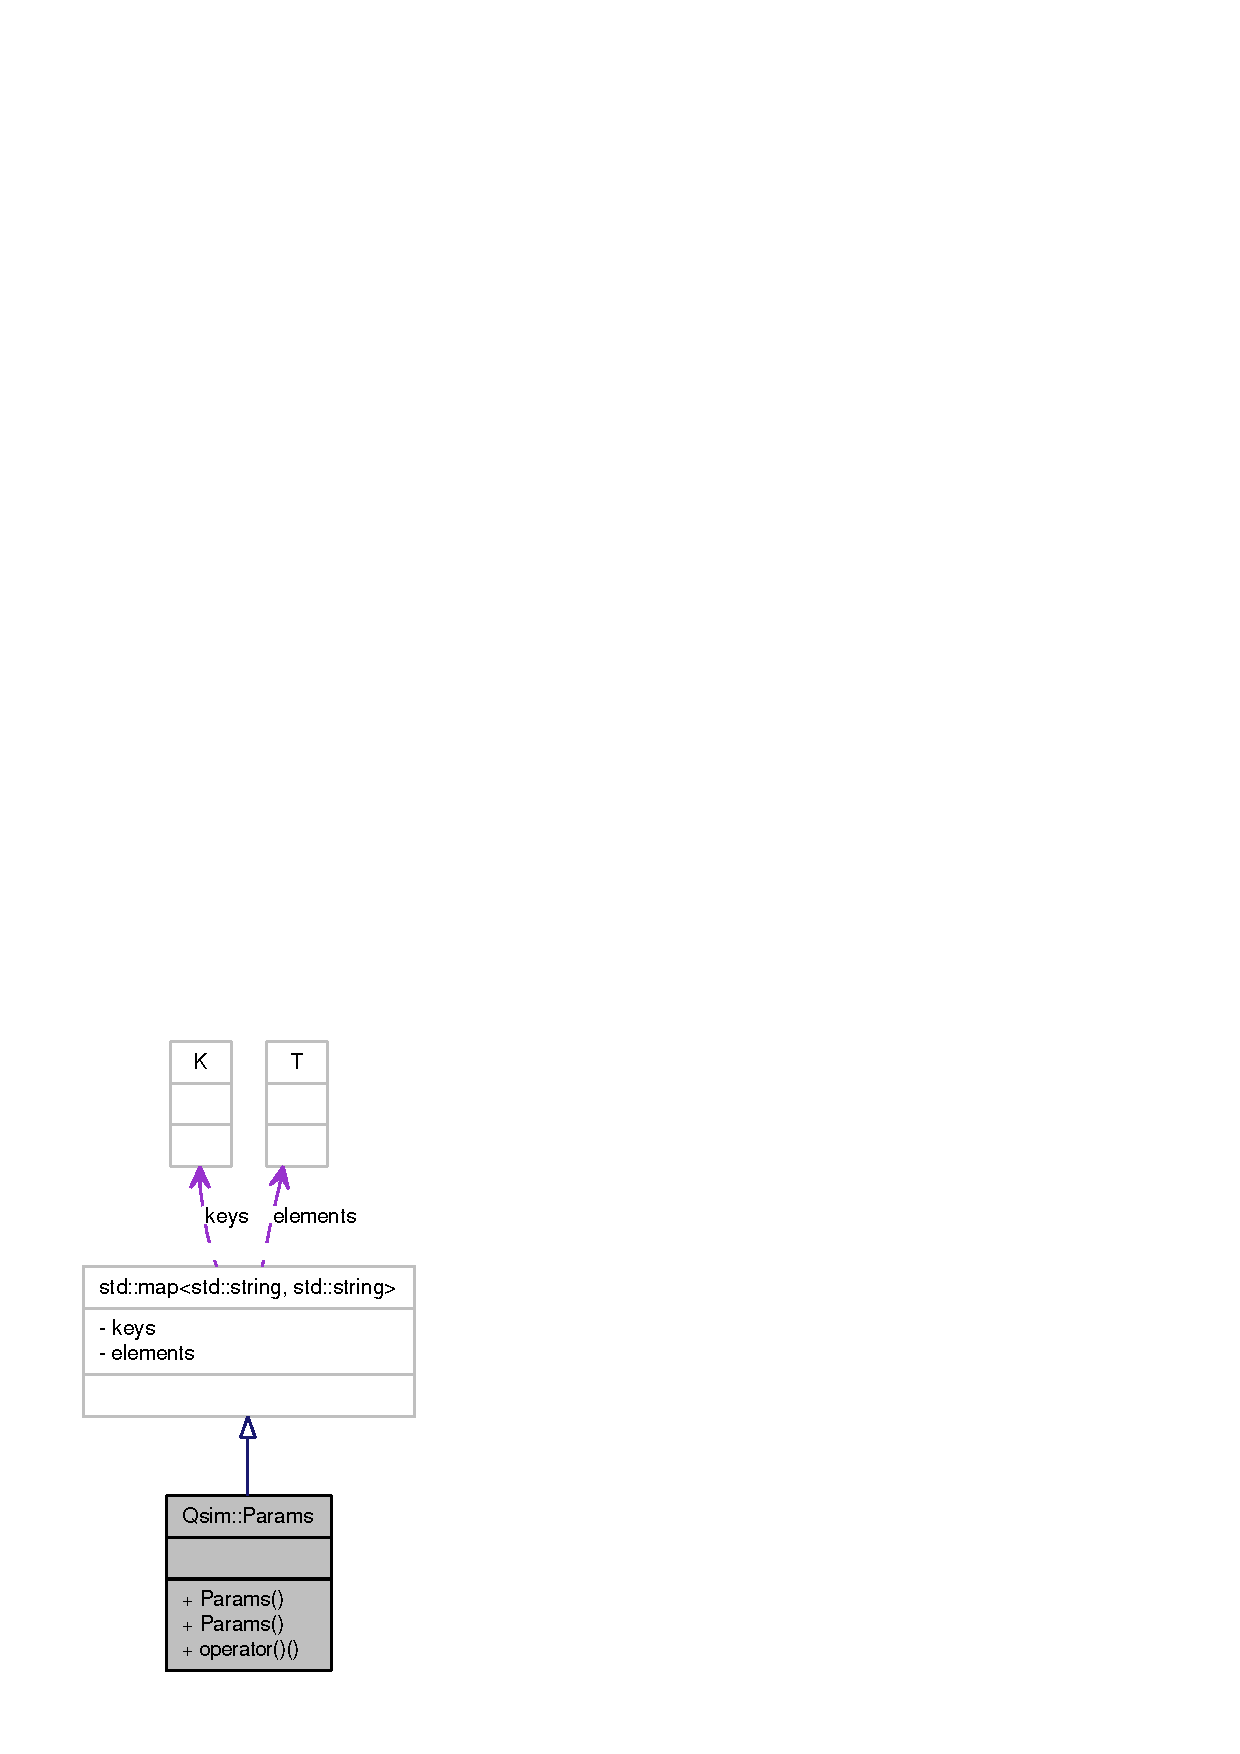
\includegraphics[width=202pt]{classQsim_1_1Params__coll__graph}
\end{center}
\end{figure}
\subsection*{Public Member Functions}
\begin{CompactItemize}
\item 
{\bf Params} ()
\item 
{\footnotesize template$<$typename T $>$ }\\{\bf Params} (std::string k, const T \&v)
\item 
{\footnotesize template$<$typename T $>$ }\\{\bf Params} \& {\bf operator()} (std::string k, const T \&v)
\end{CompactItemize}


\subsection{Detailed Description}


Definition at line 34 of file qsim.h.

\subsection{Constructor \& Destructor Documentation}
\index{Qsim::Params@{Qsim::Params}!Params@{Params}}
\index{Params@{Params}!Qsim::Params@{Qsim::Params}}
\subsubsection[{Params}]{\setlength{\rightskip}{0pt plus 5cm}Qsim::Params::Params ()\hspace{0.3cm}{\tt  [inline]}}\label{classQsim_1_1Params_94d08b6ee367ca175de49b2b1f0dadcf}




Definition at line 36 of file qsim.h.\index{Qsim::Params@{Qsim::Params}!Params@{Params}}
\index{Params@{Params}!Qsim::Params@{Qsim::Params}}
\subsubsection[{Params}]{\setlength{\rightskip}{0pt plus 5cm}template$<$typename T $>$ Qsim::Params::Params (std::string {\em k}, \/  const T \& {\em v})\hspace{0.3cm}{\tt  [inline]}}\label{classQsim_1_1Params_ffe0fe11640e589d2b6c56f8f42dffa7}




Definition at line 37 of file qsim.h.

References operator()().

\subsection{Member Function Documentation}
\index{Qsim::Params@{Qsim::Params}!operator()@{operator()}}
\index{operator()@{operator()}!Qsim::Params@{Qsim::Params}}
\subsubsection[{operator()}]{\setlength{\rightskip}{0pt plus 5cm}template$<$typename T $>$ {\bf Params}\& Qsim::Params::operator() (std::string {\em k}, \/  const T \& {\em v})\hspace{0.3cm}{\tt  [inline]}}\label{classQsim_1_1Params_2e4db64ba38696f1082ee6f3faf4b220}




Definition at line 41 of file qsim.h.

Referenced by Params().

Here is the caller graph for this function:\nopagebreak
\begin{figure}[H]
\begin{center}
\leavevmode
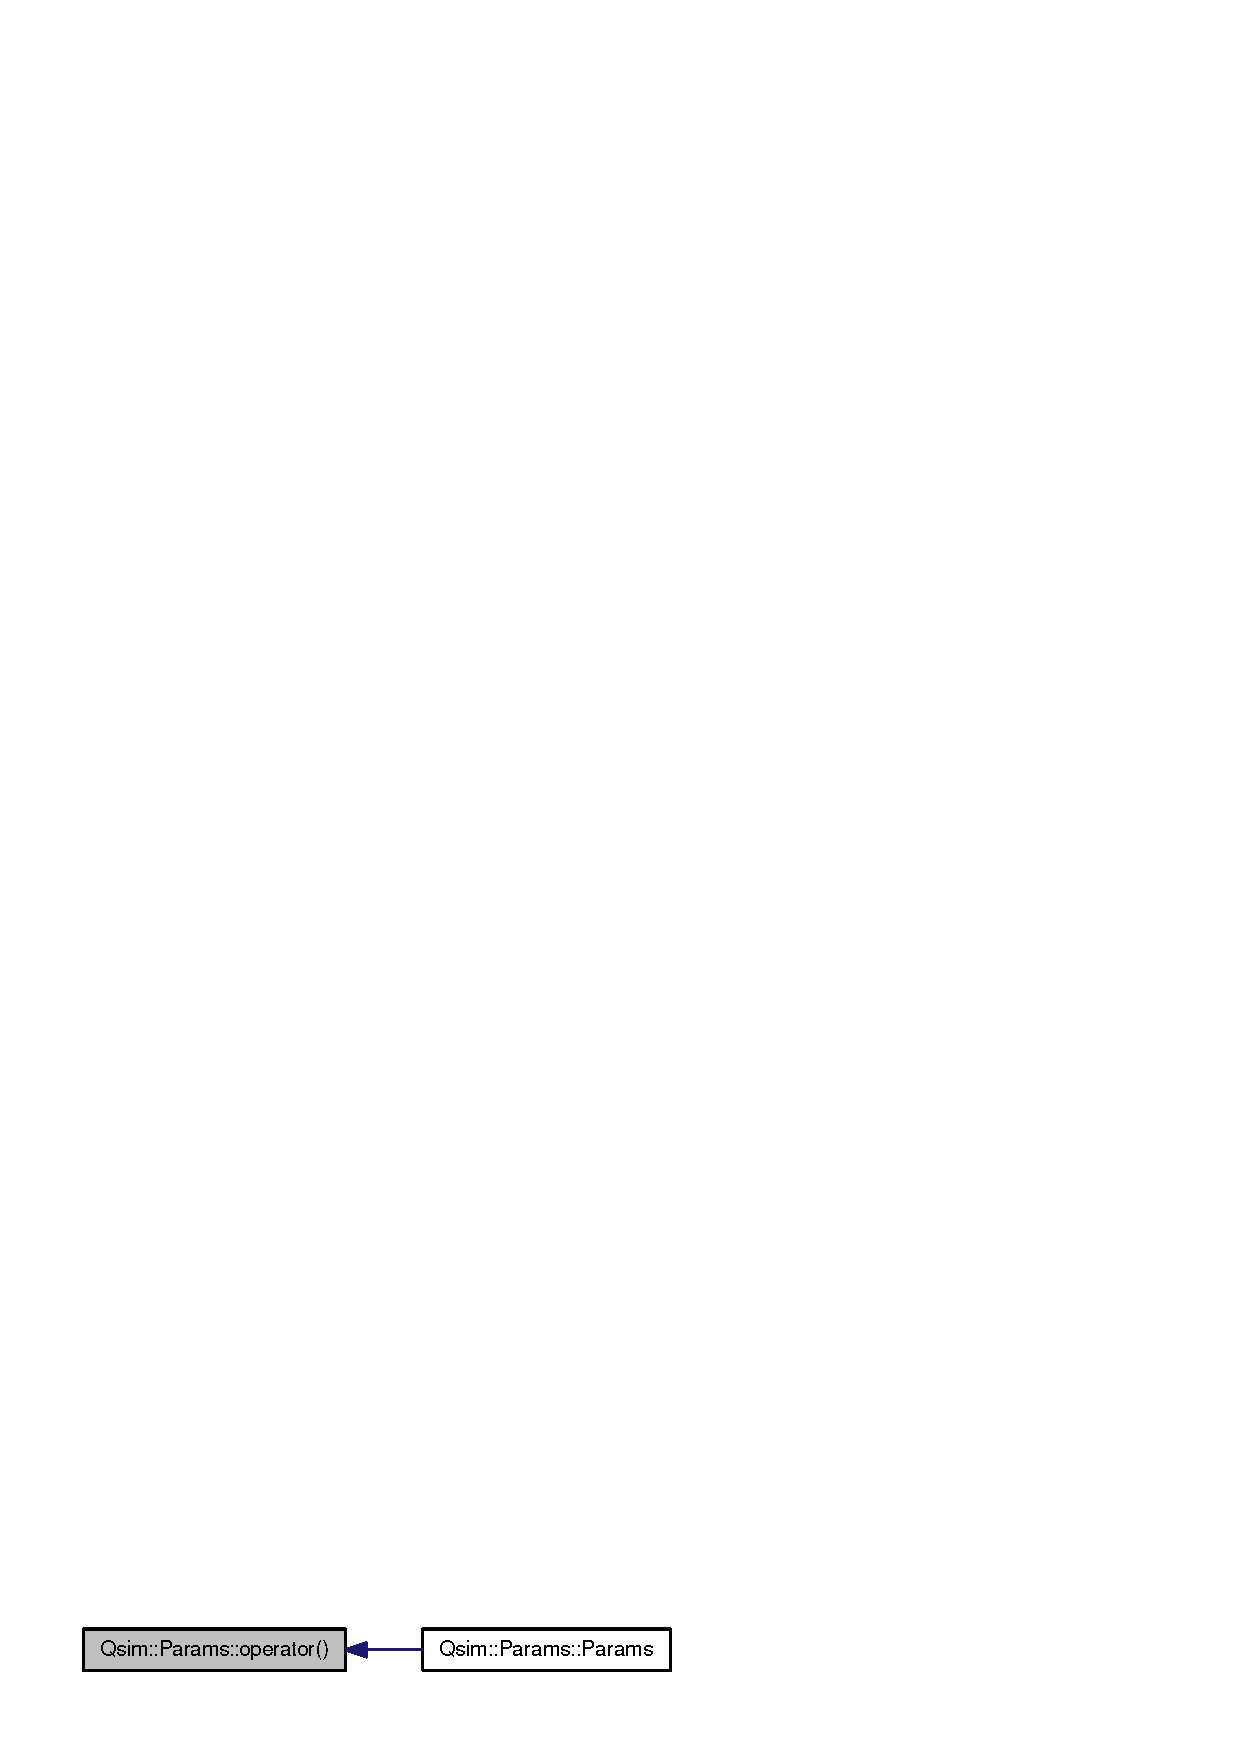
\includegraphics[width=163pt]{classQsim_1_1Params_2e4db64ba38696f1082ee6f3faf4b220_icgraph}
\end{center}
\end{figure}


The documentation for this class was generated from the following file:\begin{CompactItemize}
\item 
{\bf qsim.h}\end{CompactItemize}
